\documentclass{article}
\usepackage{tikz}
\usetikzlibrary{shapes,arrows}
\usetikzlibrary{calc}

\begin{document}

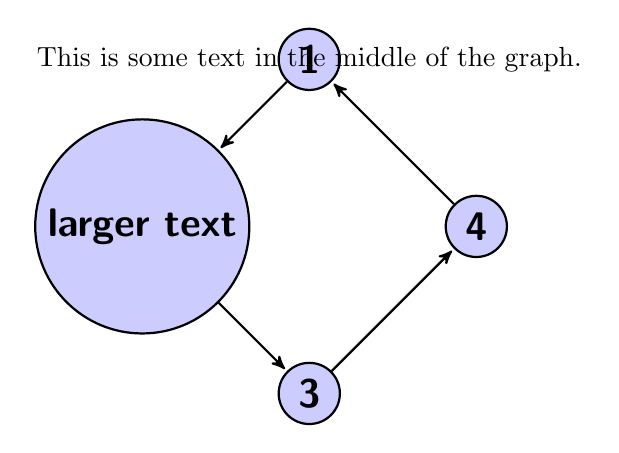
\begin{tikzpicture}[->,>=stealth',shorten >=1pt,auto,node distance=3cm,
                    thick,main node/.style={circle,fill=blue!20,draw,font=\sffamily\Large\bfseries}]

  \node[main node] (1) {1};
  \node[main node] (2) [below left of=1] {larger text};
  \node[main node] (3) [below right of=2] {3};
  \node[main node] (4) [below right of=1] {4};

\node[draw=none, fill=none] (5) {This is some text in the middle of the graph.};
  
\path[every node/.style={font=\sffamily\small}]
    (1) edge node [left] {} (2)
    (2) edge node [right] {} (3)
    (3) edge node [right] {} (4)
    (4) edge node [right] {} (1);



\end{tikzpicture}

\end{document}